\section{Problema 3}

\subsection{Primeras Consideraciones}

En un temprano intento por resolver este problema diseñamos un procedimiento que buscara el punto medio del list\'on considerado y tomara como corte \'optimo en ese instante aquel que se ubicara lo m\'as cerca del punto medio. Si bien esta idea distaba de ser correcta para el problema (se tardar\'ia un tiempo en detectar que uno de los casos de test romp\'ia este modelo), nos permiti\'o acercarnos a la idea de resolverlo mediante recursi\'on. En definitiva, la funci\'on deb\'ia tomar un liston de largo \textit{n} y un conjunto de cortes dentro de ese rango, para luego elegir uno mediante la decisi\'on explicada y luego llamar recursivamente sobre los listones \textit{$n_1$} y \textit{$n_2$}, determinados al realizar el corte, junto con los conjuntos de cortes correspondientes a cada rango. Visto de esta manera, se trataba de un enfoque \textit{Divide \& Conquer} en que la soluci\'on se ir\'ia construyendo al ir concatenando en una lista los cortes elegidos en cada llamada de la funci\'on.

\indent Pronto identificar\'iamos el err\'oneo an\'alisis de la situaci\'on y, al detectar que se trataba de un problema de optimizaci\'on un tanto m\'as complejo, acudir\'iamos a la t\'ecnica de \textit{\textsl{Programaci\'on Din\'amica}}, bajo la cual modelamos e implementamos el problema, tal como se describe a continuaci\'on. \footnote{El an\'alisis de modelado y resoluci\'on del problema mediante PD ha sido tomado y adaptado del libro: Cormen, Thomas... [et al]; \textit{Introduction to Algorithms}, Cambridge, MIT Press, 2009; (p\'ags. 359 - 390)}


\subsection{Estructura de Permutaci\'on \'Optima}

Como se ha mencionado, los parámetros de este problema son un listón de largo $n$ y un conjunto de cortes $C$ ordenados de menor a mayor, tal que además $\#C = m$.  Dejando la consideración de costo de lado, una solución a este problema estría dada por una permutación del orden de los cortes que se quieren realizar, con lo cual en principio nos encontramos con $m!$ soluciones posibles. Sin embargo, dado que cada corte conlleva un costo $q$ igual al largo del listón en que se realiza, buscamos aquella permutación tal que al realizar los cortes en ese orden la sumatoria de costos sea la mínima posible.\\
\indent Para tratar de caracterizar la solución, llamamos $Q^{s}_{ij}$ ($0 \leq i \leq j < m$) al costo de realizar en orden los cortes $c_i$,$c_{i+1}$,...,$c_j$ en un listón de tamaño $s$. El caso trivial en que $i=j$, este costo será igual a $s$. En cambio, cuando $i < j$, se debe elegir algún orden para realizar los cortes, ya que de esto dependerá cuánto costará cada uno.\\
\indent De esto último se desprende que a la hora de evaluar el costo de un conjunto de cortes, siempre debemos elegir un corte pivot $c_k$ $(i \leq k < j)$ que determina dos secciones del listón a las que quedan asociados dos conjuntos disjuntos de cortes. Luego, para determinar $Q^{s}_{ij}$ en el caso no trivial:
			\begin{itemize} \itemsep -2pt
			\item \textbf{Primero} elegimos $k / i \leq k < j$
			\end{itemize}
			\begin{itemize} \itemsep -2pt
			\item \textbf{Luego} computamos $Q^{c_k}_{ik}$
			\end{itemize}
			\begin{itemize} \itemsep -2pt
			\item \textbf{Además} computamos $Q^{s-c_k}_{k+1j}$
			\end{itemize}
			\begin{itemize} \itemsep -2pt
			\item \textbf{Finalmente} sumamos ambos costos al de haber realizado $c_k$, el cual resulta ser $s$
			\end{itemize}

A partir de este modelado salta a la vista que la solución se construye recursivamente. Habiendo determinado esto, debemos ver si entonces se cumple el \textsl{Principio de Optimalidad}.\\
\indent Supongamos que encontramos el valor mínimo de $Q^{s}_{ij}$ tomando como corte pivot $c_k$ para algún $k$ entre $i$ y $j$. Luego por lo expuesto antes necesariamente el valor de la subsolución $Q^{c_k}_{ik}$ del subproblema deberá ser óptimo, ya que si existiera otro orden para obtener un costo más barato, entonces la solución inicial no habría sido la óptima. Lo mismo sucede al considerar el subproblema derecho. El absurdo proviene de que $Q^{s}_{ij} = Q^{c_k}_{ik} + s + Q^{s-c_k}_{k+1j}$, luego si la solución es óptima la suma de los términos que la conforman también debe serlo, lo cual se traduce en que las subsoluciones de los subproblemas determinados sean también óptimas.\\
\indent Se ve entonces que cualquier instancia no trivial del problema de optimización de los cortes requiere que se separe el problema en dos subproblemas, y que a partir de la óptima resolución de ellos podemos construir una solución óptima a nuestro problema. Es importante notar que se deben recorrer todos los posibles cortes pivot en una instancia dada para asegurarse que se eligió cortar de manera óptima.\\

\subsection{Solución Recursiva}

Para este problema podemos determinar la solución óptima recursivamente al ir combinando soluciones óptimas de los subproblemas determinados. En particular, se debe organizar el orden de los cortes en el listón en función de su costo. Es decir que la función que implementamos toma decisiones en base a esta variable, pero el objetivo ulterior no es devolver el costo final sino cierta permutación de cortes asociada a ese costo. Para ello entonces operamos también con una lista donde iremos agregando los cortes desde el primero al últimoq ue se realiza.\\

\indent Sea $P[i,j,s]$ la permutación de cortes asociada al valor óptimo $Q^{s}_{ij}$, luego la solución del problema estará dada por $P[0,m-1,s]$. La lista $P$ la definimos recursivamente de la siguiente manera:
			\begin{itemize} \itemsep -2pt
			\item Si $i = j$ el problema es trivial, pues sólo se realiza un corte en el listón s, con lo cual $P[i,j,s] = \{c_i\}$.
			\end{itemize}
			\begin{itemize} \itemsep -2pt
			\item Si $i < j$ debemos seguir lo expuesto antes y pensar que primero se realiza el corte pivot y luego se realizan 				los cortes de manera óptima sobre el sublistón izquierdo y de la misma manera sobre el sublistón derecho. Notar que 				es indistinto el orden en que se ponga el bloque izquierdo o derecho. De esta manera $P[i,j,s] = \{c_k\} ++ P[i,k,c_k] 				++ P[k+1,j,s-c_k]$.
			\end{itemize}

Sin embargo este modelo de recursión asume que se conoce cuál es el corte pivot que garantiza la solución óptima. En realidad, ese k debe ser elegido en función de la permutación que genere el mínimo costo. Como complemento a lo anterior llamamos $Q[i,j,s]$ al mínimo costo al realizar los cortes $c_i$ hasta $c_j$ en el listón de tamaño $s$, el cual también se define recursivamente de la siguiente manera:
	\[ Q[i,j,s] = \left\{ \begin{array}{ll}
		 s & \mbox{if $i = j$};\\
		\min_{i \leq k < j} \{ Q[i,k,c_k] + Q[k+1,j,s-c_k] \} + s & \mbox{if $i < j$}.\end{array} \right. \] 

	
Aunque se trate de dos funciones recursivas distintas, se podrá observar que están intimamente ligadas. En términos implementativos se trata simplemente de una sola función que evalúa costos y en vez de devolver este retorna la permutación de cortes que utilizó para llegar al mismo.\\

\indent Otra observación que debe hacerse es que en este análisis se pasó por alto el hecho de que, al seccionar el listón, estas funciones teóricas sólo recuerdan el tamaño, pero no los extremos relativos a las posiciones desde donde fue seccionado el listón original. De esta manera, en este análisis teórico estaríamos evaluando realizar el corte $c_i = 7$ en un listón cuyos extremos son 0 y 3 pero que ubicado en el listón original sus extremos serían 5 y 8. Esta omisión se da ya que sólo volvería engorroso el planteo de las funciones, pero desde ya es algo que sí se contempla en la función implementada.

\subsection{Calculando las Subsoluciones}

¿Qué sucede a la hora de calcular las diversas subsoluciones de los subproblemas que se van planteando? Hasta aquí sólo se ha modelado una forma recursiva para resolver el problema, teniendo en cuenta que éste cumple el principio de optimalidad. ¿Pero acaso es esto mejor que la fuerza bruta, o backtracking, donde podríamos evaluar todas las permutaciones posibles? La respuesta es, por el momento, no. En la Figura ~\ref{fig:overl} vemos un esquema del árbol de problemas que se va generando al evaluar el modelo recursivo antes descripto, llamando a $P[1,4,s]$. Se puede ver fácilmente como en diversos llamados de la función recursiva se repiten los subproblemas, lo cual implica que la función planteada hasta el momento debe resolver varios cómputos repetidas veces. Esta característica, \textsl{superposición de subproblemas}, es esencial para una solución de Programación Dinámica. A diferencia de un problema que se pudiera resolver con Divide \& Conquer, en que se generan nuevos y disjuntos subproblemas, aquí vemos como en realidad el espacio de subproblemas distintos es reducido.\\
\begin{figure}[h]
\centering                                                       
        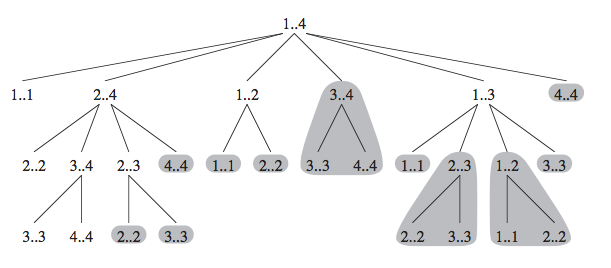
\includegraphics[width=320pt]{./figs/p3overlapping.png}
	\caption{Se ve la superposición de subproblemas, y como los pintados en gris serían buscados en una tabla y no calculados. \textsl{Fuente: Cormen..., p(385)}. }
	\label{fig:overl}
\end{figure}
\indent Es posible ver que implementar directamente una solución basada en el modelo tal cual fue planteado hasta aquí tomaría tiempo exponencial respecto de $m$ \footnote{Si bien escapa a nuestro foco de análisis, puede encontrarse una demostración para el análogo problema de producto de matrices en \textit{Cormen...} (p. 386)}. Es así que el último ingrediente agregado a este modelo es una tabla o diccionario que recordará aquellos subproblemas calculados para que en caso de requerir una solución precomputada esté disponible en tiempo constante. De esta manera nuestra solución al problema es un algoritmo recursivo, \textsl{top down} ya que va partiendo los problemas grandes en subproblemas más pequeños, pero que a diferencia de la ineficiente versión original va 'recordando' o \textsl{memoizando} las soluciones para que otras ramas de las llamadas recursivas no tengan que recalcular lo mismo nuevamente. Más adelante, en el análisis de complejidad de nuestro algoritmo, se verá cuán importante es la mejora al introducir la \textsl{memoización} en términos de tiempo de cómputo (no así de memoria).

\subsection{Estructuras}

Antes de analizar el algoritmo implementado y evaluar su complejidad, es importante realizar un breve análisis de las estructuras usadas para la resolución del problema.\\

\textbf{Listón.} Decidimos crear la estructura Listón para así tener alojados no sólo los datos iniciales del problema (lista de cortes, tamaño) sino también la tabla de soluciones (parciales en la mayor parte de los casos) computadas a lo largo de la ejecución. De esta manera contenemos toda la información en un mismo objeto al que se accede y se modifica en las distintas llamadas de la recursión, mientras que lo único que cambia en las mismas es el pasaje de los parámetros que determinan qué sublistones se mirarán dentro de ese listón (esto se analiza luego en la función correspondiente).\\
\indent Los campos de Listón: el tamaño es un entero, mientras que los cortes se guardan en un arreglo. El diccionario de soluciones no es otra cosa que una matriz o tabla. Dado que los métodos de Listón, salvo el constructor, son simplemente acceder a estos campos, se ve sin dificultad que tienen complejidad $O(1)$. En cambio, el constructor debe crear la matriz e inicializar la mitad de ella con el valor $\infty$ para indicar que todavía no se han insertado soluciones en esos casilleros. Por lo tanto, la complejidad del mismo es $O(m^2)$. El significado del contenido de la tabla y el por qué de cómo está indexada se ve a continuación.\\

\textbf{Solución.} Esta estructura es una tupla, con la semántica de una 'solución' al problema. La definimos de esta manera ya que como primera componenete tiene un costo, y como segunda una lista (implementada sobre la interfaz de Java \textsl{List$<T>$} sobre la clase \textsl{ArrayList$<T>$}). El vínculo entre ambas componentes es que el costo corresponde a haber realizado los cortes de la lista, en ese orden, en algún sublistón. A diferencia del modelo teórico planteado antes, aquí no guardamos ninguna relación con el tamaño del listón. Esto es porque en realidad el valor de $Q^{s}_{ij}$ es único en función de $i$ y $j$; nunca se dará una situación en que se quiera calcular $Q^{s}_{ij}$ y $Q^{t}_{ij}$ con $ s \neq t$. Por ello, la tabla de 'memoización' está indexada en base a los índices de corte $i,j$, y en definitiva es por ello que se produce la mencionada superposición de subproblemas.\\
\indent La complejidad de ambos constructores es constante. Por un lado el constructor vacío \textit{Solucion()} se trata de una asignación de un campo entero y la creación de un ArrayList vacío, lo cual crea una lista en base a un arreglo con capacidad para 10 elementos. Por el otro lado, el constructor que toma dos enteros realiza también una asignación a un campo y además de crear una lista vacía, le agrega el otro entero de la entrada (lo cual es, amortizado, O(1)).\\
\indent Por último, esta clase tiene otra operación llamada \textit{Combinar(Solucion,Solucion,int,int)}. Si llamamos $s1$ y $s2$ a las soluciones de entrada, entonces la complejidad de esta operación es O($max$($\#$s1.cortes, $\#$s2.cortes)), ya que luego de crear la lista vacía, primero agrega el corte individual que vino en la entrada, y luego agrega (concatena) los cortes de s1, para luego agregar los de s2. Dado que agregar $n$ elementos demanda O($n$), la complejidad estará por la máxima cantidad de cortes que se encuentre entre las dos soluciones. Si tenemos en cuenta que se trata de subconjuntos de la cantidad de cortes inicial, la complejidad de peor caso de esta operación será O($m$).\footnote{Las complejidades de las clases de Java fueron tomadas de http://docs.oracle.com/javase/6/docs/api/}

\subsection{PSeudocódigos y Complejidades}

\begin{algorithm}
\caption{cortarListon (\textbf{in/out} liston: \textsl{Liston}) $\rightarrow$ res: \textsl{Solucion}}
\begin{algorithmic}[1]

\STATE $ m \leftarrow liston.cantCortes()$
\STATE $ solucion \leftarrow memoizedCosto(liston,0,m-1,0,liston.largo()$
\RETURN $solucion$

\end{algorithmic}
\end{algorithm}

\begin{algorithm}
\caption{memoizedCosto (\textbf{in/out} liston: \textsl{Liston}, \textbf{in} i,j,izq,der: \textsl{int}) $\rightarrow$ res: \textsl{Solucion}}
\begin{algorithmic}[1]

\IF{ $i == j$}
	\IF{ $liston.dameCorte(i) == izq || liston.dameCorte(j) = der$ }
		\STATE $corteInvalido \leftarrow Solucion()$
		\STATE $liston.insertarSolucion(i,j,corteInvalido)$
		\RETURN $corteInvalido$
	\ELSE
		\STATE $corteBase \leftarrow Solucion(der-izq, liston.dameCorte(i))$
		\STATE $liston.insertarSolucion(i,j,corteBase)$
		\RETURN $corteBase$
	\ENDIF
\ELSE
	\STATE $costoAnt \leftarrow \infty$
	\FOR{$k = i$ \textbf{to} $j-1$} 
		\IF{ $not(liston.haySolucion(i,k)$}
			\STATE $memoizedCosto(liston,i,k,izq,liston.dameCorte(k))$
		\ENDIF
		\STATE $solIzq \leftarrow liston.dameSolucion(i,k)$
		\IF {$not(liston.haySolucion(k+1,j)$}
			\STATE $memoizedCosto(liston,k+1,j,liston.dameCorte(k),der)$
		\ENDIF
		\STATE $solDer \leftarrow liston.dameSolucion(k+1,j)$
		\STATE $costoAct \leftarrow solIzq.costo + solDer.costo + (der-izq)$
		\IF {$costoAct < costoAnt$}
			\STATE $costoAnt \leftarrow costoAct$
			\STATE $ktemp \leftarrow k$
			\STATE $sol_ij \leftarrow combinar(solIzq,solDer,costoAct,ktmp)$
		\ENDIF
	\ENDFOR
	\STATE $liston.insertar(i,j,sol_{ij})$
	\RETURN $sol_{ij}$
\ENDIF
\end{algorithmic}
\end{algorithm}

\indent La primera función, \textsl{cortarListon}, hereda su complejidad de \textsl{memoizedCosto}, ya que la instrucción de la primera línea es simplemente O(1).\\
\indent La complejidad de \textsl{memoizedCosto} es un tanto más compleja de calcular, ya que se trata de una función recursiva. Supongamos por el momento que es $T(m)$. La propuesta para este análisis es primero hacer un desglose de las complejidades de cada línea, y luego ver de qué manera repercute esto en la recursión y cuál es finalmente la verdadera complejidad de la función.\\
\indent Si dividiéramos en bloques la función, el primero estaría comprendido entre la línea 1 y la línea 10, representando el análisis de casos base. Todas las operaciones en este bloque, por lo justificado en la sección anterior sobre los métodos de las estructuras, es O(1).\\
\indent El segundo bloque, el cual va de la línea 12 a la 28, comprende casi la mayor parte de la función, y es el que se ocupa de verificar qué corte se debe realizar en esa llamada, actualizar la tabla de memoización y devolver una solución parcial. Salvo una asignación en O(1) al principio, el resto del bloque está comprendido por un sub-bloque iterativo. Supongamos que la complejidad de lo que se ejecuta en ese bloque es $T(F)$. Luego, como el ciclo itera entre $i$ y $j$, y estos a su vez están comprendidos entre $0$ y $m-1$, la complejidad de este bloque sería O($m * T(F)$). Ahora bien, veamos cuál es la complejidad dentro del ciclo.\\
\indent Aquí es donde se produce el truco de la memoización, que nos ahorrará operar en tiempo exponencial (como se mostró antes) para llegar, idealmente y según veremos en pocas líneas, a tiempo polinomial. Tanto en las líneas 14-17, como 18-21, la función parte en el listón en el $k$-ésimo corte y luego busca en la tabla los costos de lo que queda a izquierda y a derecha. Si nunca lo calculó, deberá hacerlo mediante la recursión. Supongamos para el análisis que siempre encuentra la solución en la tabla. Entonces, hasta aquí, la complejidad dentro del ciclo es constante. Luego hace algunas cuentas con enteros y comparaciones, para en la línea 26 utiliza el método combinar, que según probamos en las estructuras demanada O($m$). De esta manera, con la suposición de que siempre encuentra los valores en la tabla, la complejidad del ciclo es O($m * m$), o sea O($m^2$). Finalmente la penúltima línea inserta la solución parcial en tiempo constante y la devuelve.\\
\indent Suponiendo que los valores pedidos siempre están en la tabla (se acceden entonces en O(1)), llegamos a que $T(m) = O(m^2)$. Pero la realidad es que nuestra suposición no es del todo correcta, ya que al menos hay $m$ casos en los que para esos cortes se deben computar los subproblemas izquierdo y derecho por primera vez, con lo cual en realidad la complejidad es O($m * m^2$), lo que \textbf{finalmente da en el orden de} O($m^3$).

\subsection{Análisis Toma de Tiempos}

\indent Para correr el algoritmo, hicimos 1000 corridas de cada caso para poder tener un tiempo estimativo en milisegundos, dado que si corrìamos una sola vez los casos, el tiempo era insignificante (para poca cantidad de cortes).\\
\indent A continuacion presentamos el grafico obtenido para un liston de tamaño 200 variando el parámetro $m$ (cant. de cortes) entre 3, 6, 10, 15, 19, 27 y 36:
\begin{figure}[h]
\centering                                                       
        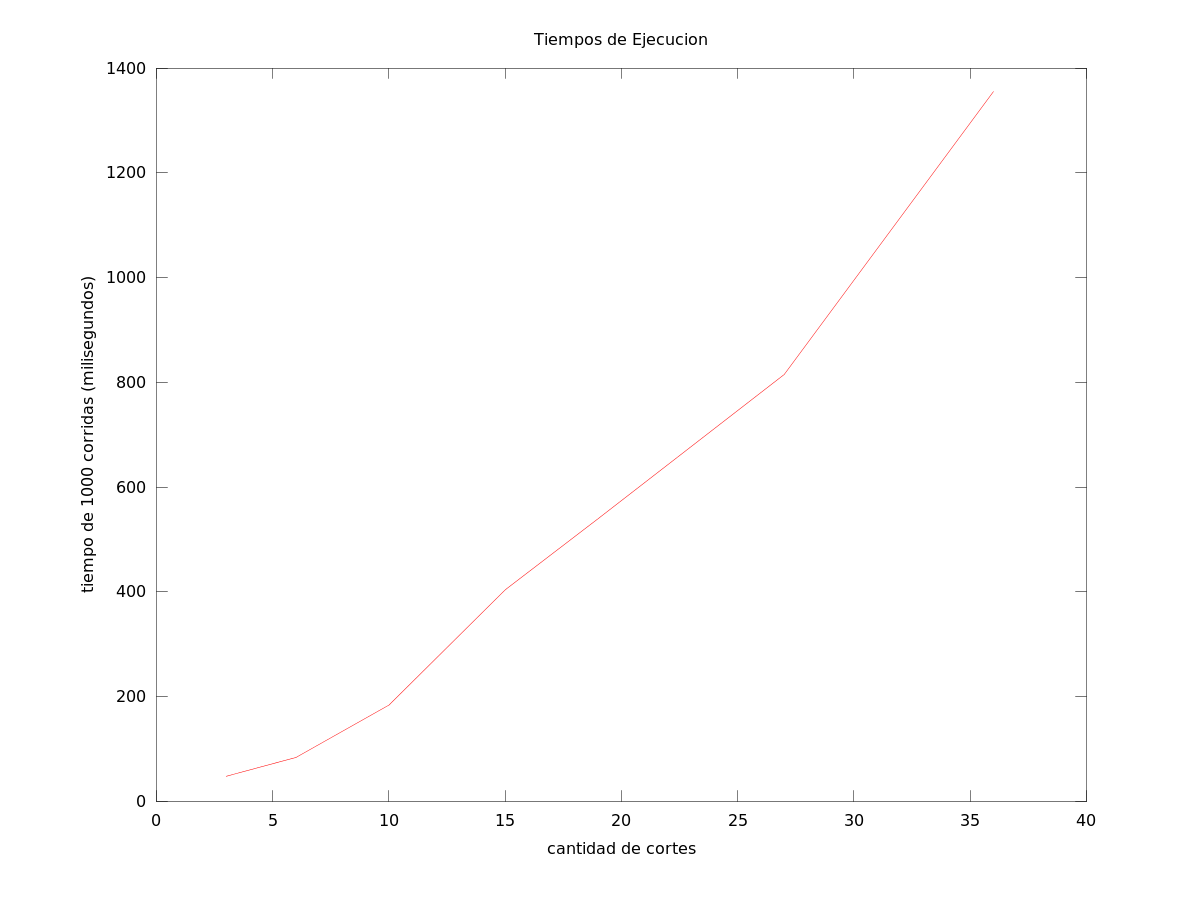
\includegraphics[width=320pt]{./figs/p3tiempos.png}
	\caption{En este gráfico se ejemplifican algunas corridas para cierta cantidad de cortes}
	\label{fig:p3tiempos}
\end{figure}
\indent Al realizar el gràfico, nos llevamos la sorpresa de que la gràfica resultante parecìa no ser cúbica. Luego de realizar varias pruebas notamos que el comportamiento de los tiempos que obteníamos no era tan regular como esperábamos (a diferencia por ejemplo del primer problema). Si bien no sabemos con certeza a qué atribuirlo, algunas de las hipótesis con que contamos es que la metodología para contar los tiempos no fuera la correcta, o que no hubieramos dispuesto una distribución uniforme de los casos de prueba. Esto es, si bien variamos el parámetro $m$, desconocemos qué relación puede existir con la longitud del listón. Si bien por el modelado y el análisis expuesto esto no infiere directamente, podría ser que lo haga la densidad o distribución de cortes dada la superficie del listón.\\
